
\subsection{Ontología del dominio} \label{sec:ontologia}

El conocimiento adquirido para este problema se representa mediante una
ontología. En esta aparecen todos los conceptos detallados en la
\autoref{sec:conceptualizacion} y las relaciones entre ellos, puesto que debe
permitir al sistema basado en el conocimiento razonar sobre ellos de forma
adecuada. Para formalizarlos, deberemos pensar en una forma para representarlos
y que nuestro sistema basado en el conocimiento lo entienda. A continuación, 
pasamos a detallar las partes principales de la ontología desarrollada.

La ontología empieza con la clase \texttt{Alumno}, cuyas instancias se podrán 
identificar por su atributo \texttt{id} (correspondiente al DNI del alumno).
Desde un alumno podremos acceder a todo su expediente de las asignaturas a las
que se ha presentado y a sus preferencias sobre cómo le gustaría que fuese su
próxima elección de matrícula. Esto nos sirve para que, desde la clase 
\texttt{Alumno}, podamos gestionar sus preferencias y restricciones o 
inferirlas si es necesario y así poder escoger las mejores asignaturas para 
una buena recomendación. Por ello, en la ontología tenemos las clases 
\texttt{Expediente}, \texttt{ResPref} y \texttt{Recomendacion} asociadas a 
la clase \texttt{Alumno}: con el conocimiento del expediente y de las 
restricciones y preferencias, construiremos la recomendación.
La parte de la ontología asociada al alumno y a sus 
conceptos asociados se muestra en la \autoref{fig:ontologia-alumno}.

\begin{figure}[ht]
    \centering
    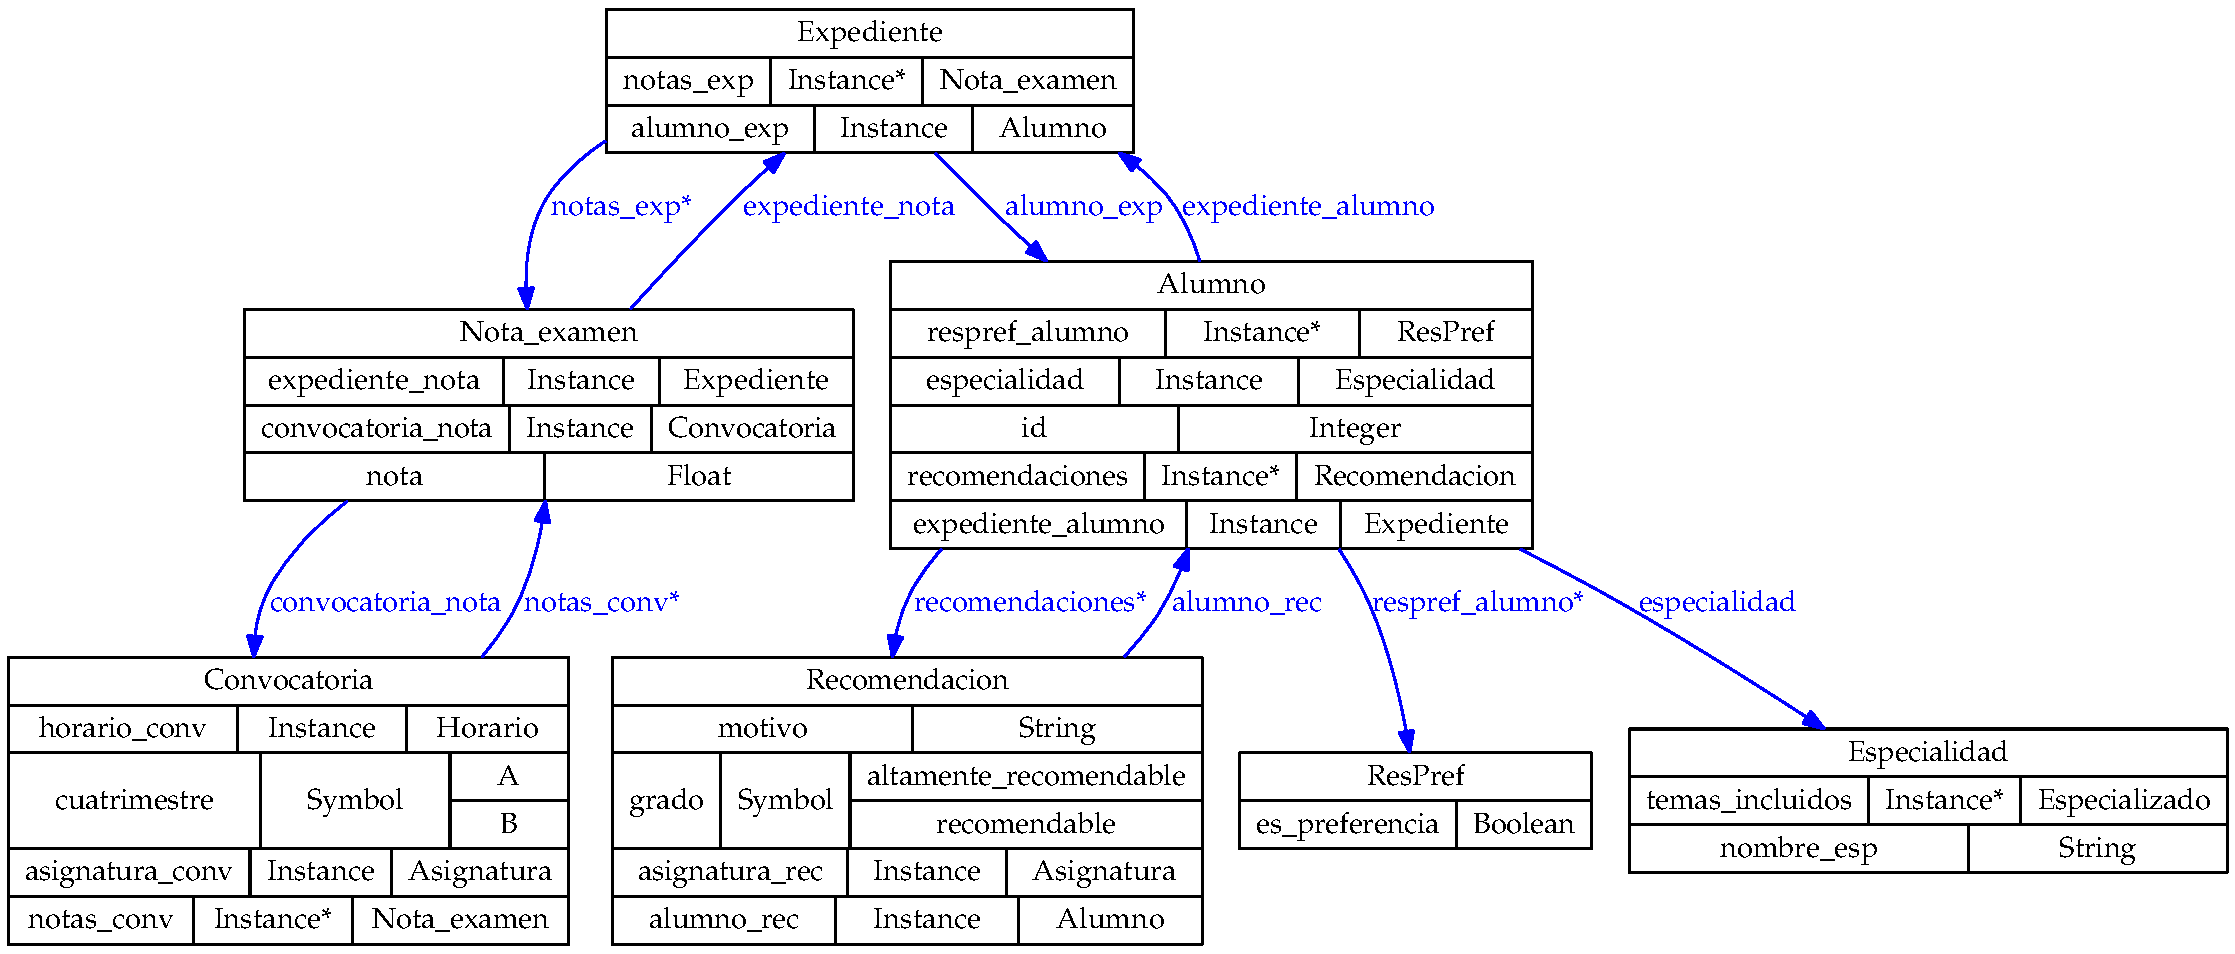
\includegraphics[width=15cm]{ontologia-alumno}
    \caption{Representación gráfica de la parte de la ontología 
        correspondiente a los alumnos.}
    \label{fig:ontologia-alumno}
\end{figure}

El expediente único del alumno almacenará los resultados de todas las 
convocatorias de exámenes del alumno. Para distinguir una convocatoria 
usaremos la asignatura y el cuatrimestre en el que se ha presentado. Esto nos 
permitirá que un alumno se pueda presentar a la misma asignatura en más de una 
ocasión si éste la suspendiera. Se asocia, pues, la clase \texttt{Expediente} 
a una clase \texttt{Nota\_examen} que almacena la nota en un atributo 
\texttt{nota} y, a su vez, está asociada a la clase \texttt{Convocatoria}, 
a partir de la cual se puede recuperar el resto de la información de la 
convocatoria: de qué asignatura se trata y el cuatrimestre y el horario en los 
que se cursó. 

Las asignaturas son los conceptos que permanecerán estáticos durante toda
la ejecución del sistema. El conocimiento asociado a estas no podrá ser 
modificado por el alumno porque es independiente de él y es algo nos 
proporciona la FIB. Cada asignatura consistirá en un nombre (tomaremos sus 
siglas para abreviar), el curso en el que aparece en el plan de estudios, su 
número de créditos ECTS (así como la distribución en horas de esta carga por 
los conceptos de teoría, problemas y laboratorio), el horario de impartición y 
si la asignatura consiste en un proyecto. También incluirá las estadísticas 
más recientes referentes al número de alumnos matriculados y el porcentaje de 
aprobados; y la relación de la asignatura con las competencias que desarrolla 
y con los temas en los que se ubica su contenido. Además, modelamos para cada 
asignatura las dependencias con otras asignaturas en forma de prerrequisitos
(las asignaturas que se deben haber aprobado previamente a esta matrícula), 
correquisitos (las asignaturas que se deben haber aprobado previamente a esta 
matrícula o bien matricularlas conjuntamente), precorrequisitos (las 
asignaturas que se deben haber matriculado previamente a esta matrícula) 
y orrequisitos (conjuntos de asignaturas al menos una de las cuales se debe 
haber aprobado previamente a esta matrícula). 

\begin{figure}[ht]
    \centering
    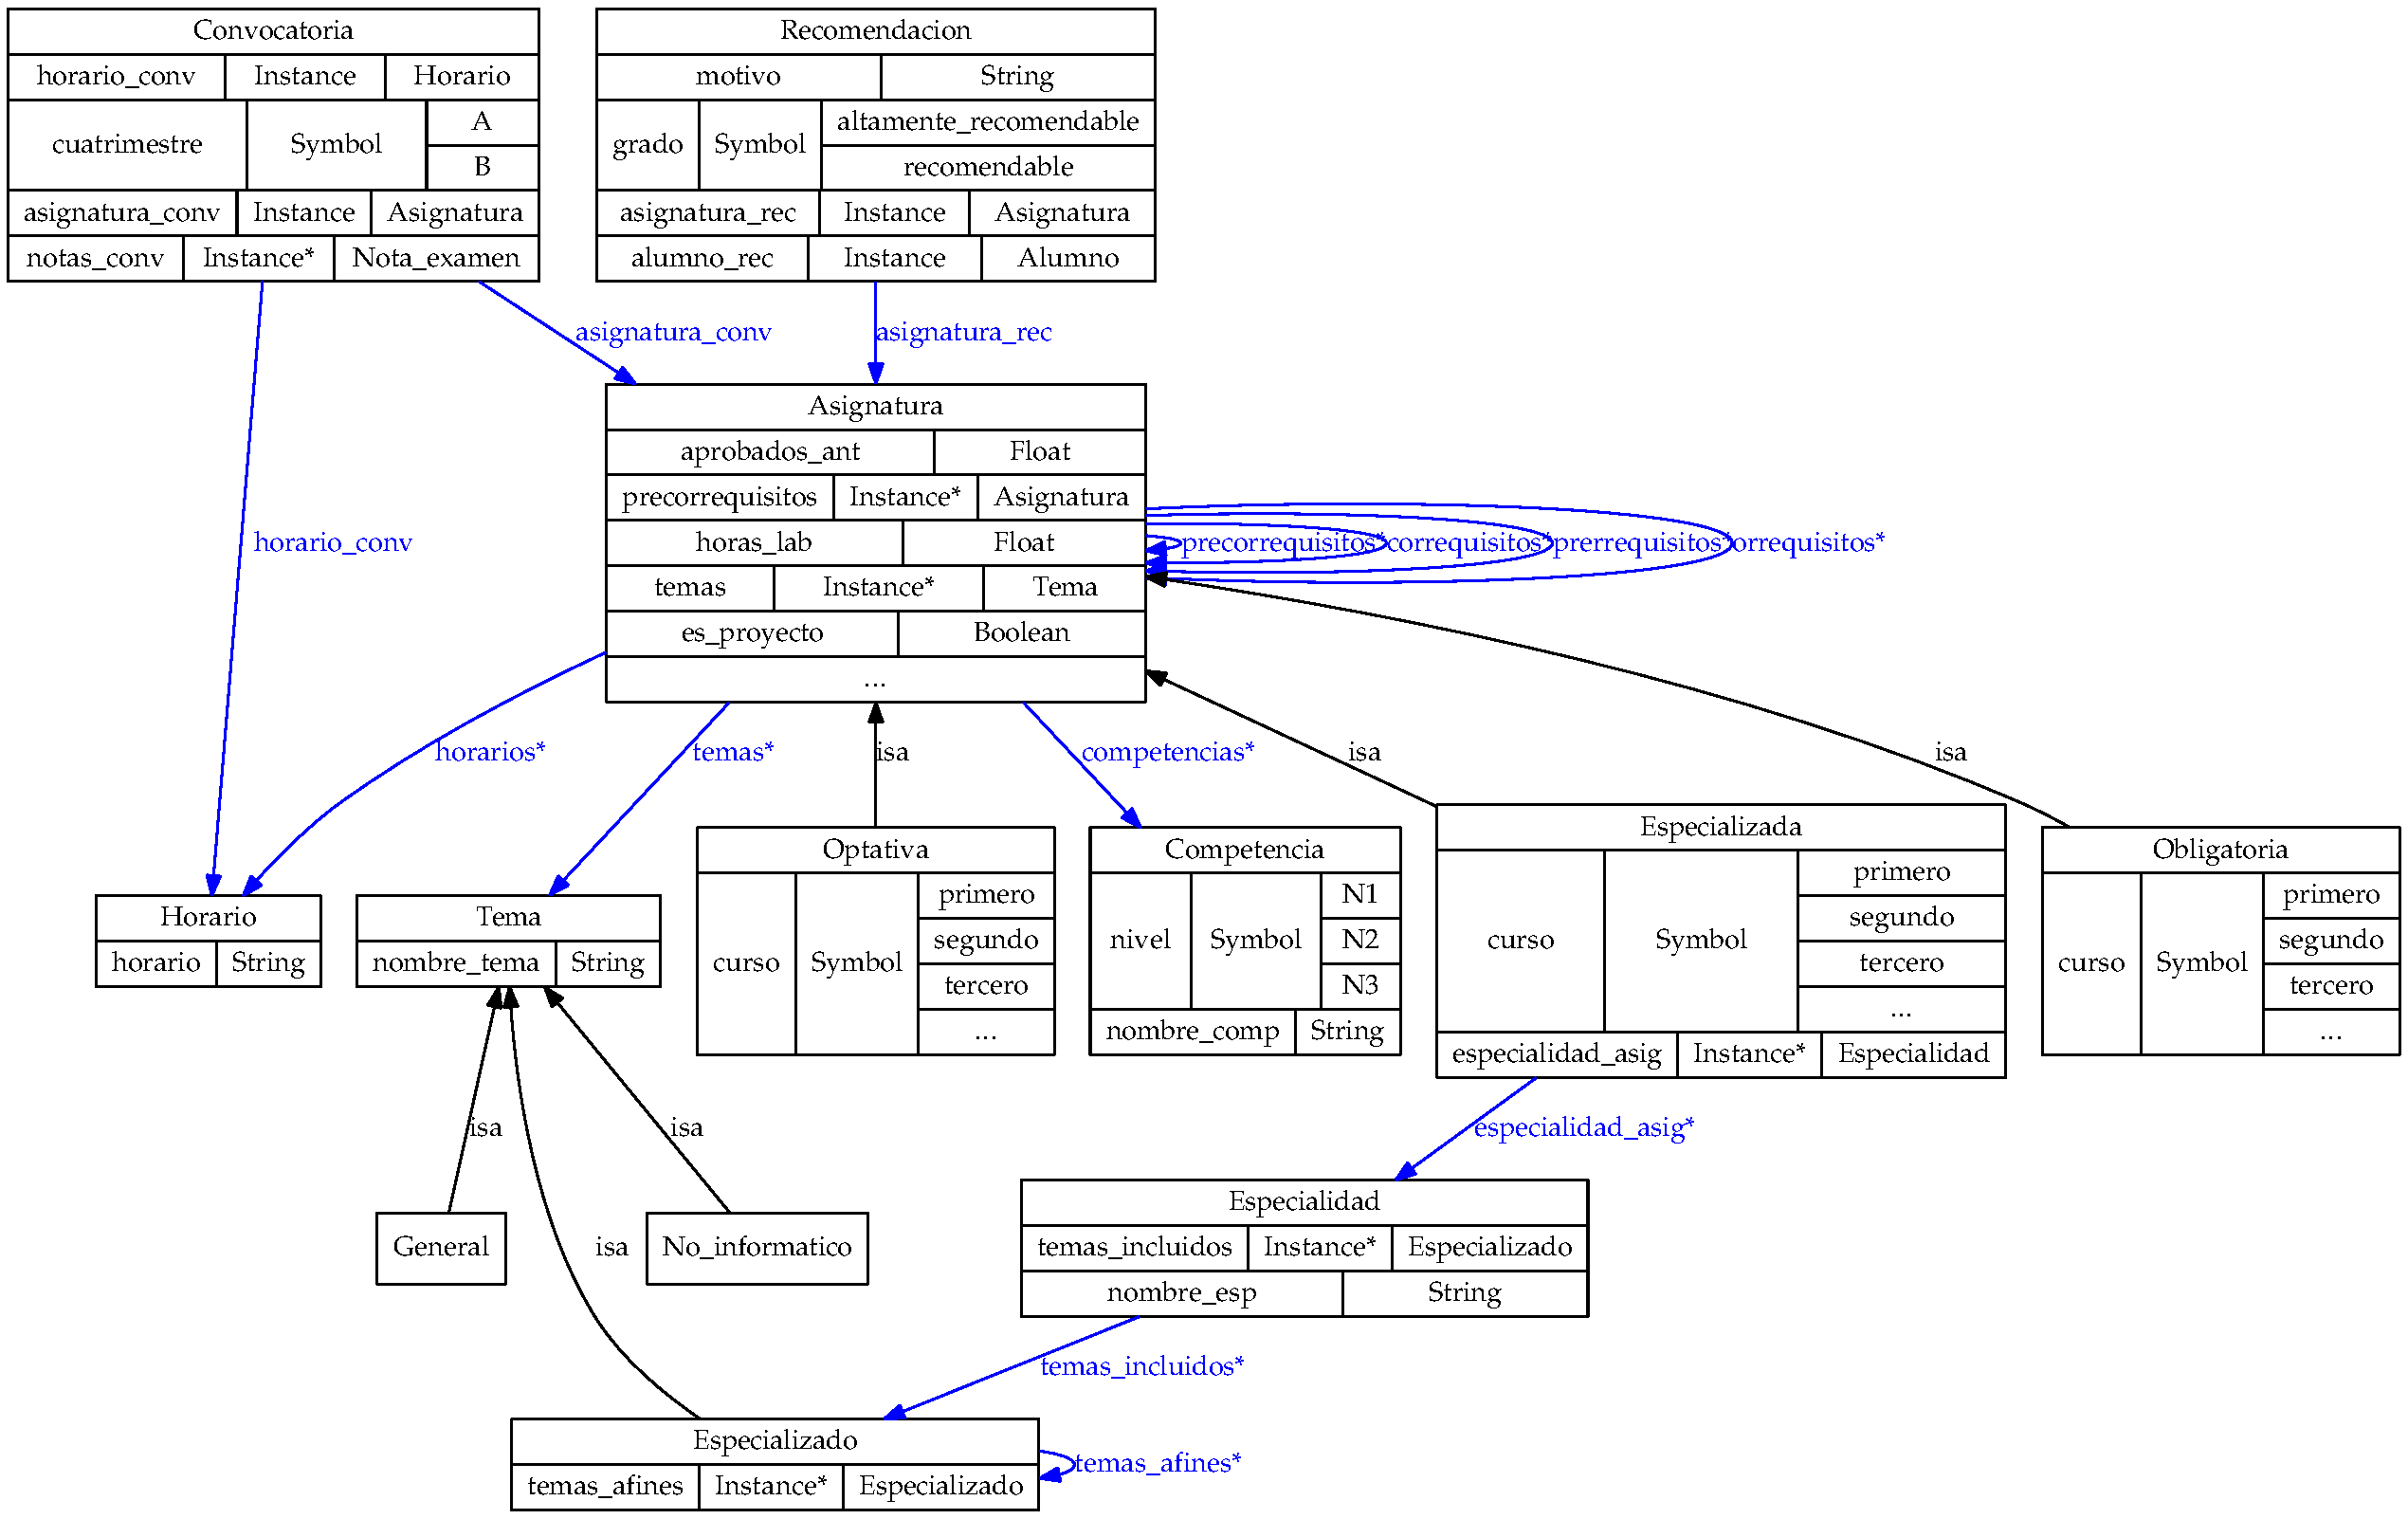
\includegraphics[width=15cm]{ontologia-asignaturas}
    \caption{Representación gráfica de la parte de la ontología 
        correspondiente a las asignaturas.}
    \label{fig:ontologia-asignaturas}
\end{figure}

Así, pues, se tiene una clase \texttt{Asignatura} con los atributos 
\texttt{nombre}, \texttt{curso}, \texttt{num\_creditos}, 
\texttt{horas\_teoria}, \texttt{horas\_prob}, \texttt{horas\_lab}, 
\texttt{es\_proyecto}, \texttt{matriculados\_ant} y \texttt{aprobados\_ant} y 
relacionada con las clases \texttt{Horario} (de la cual habrá dos instancias: 
el horario de mañana y el horario de tarde), \texttt{Competencia} (que 
representa las competencias transversales) y \texttt{Tema} (que representa 
los temas tratados en la asignatura), así como cuatro relaciones 
\texttt{prerrequisitos}, \texttt{correquisitos}, \texttt{precorrequisitos} y 
\texttt{orrequisitos} consigo misma. Todos estos atributos y asociaciones son 
la forma de representar el contenido descrito en el párrafo anterior. Por 
otro lado, de la clase \texttt{Asignatura} se derivan tres clases que 
representan los diferentes tipos de asignaturas del plan de estudios: 
\texttt{Especializada} para las asignaturas de especialidad (contiene un 
atributo adicional que indica la especialidad a la que pertenece), 
\texttt{Obligatoria} para las asignaturas troncales y \texttt{Optativa} para 
las asignaturas de carácter opcional. 

La clase \texttt{Convocatoria} mencionada anteriormente también está 
asociada con \texttt{Asignatura} y con \texttt{Horario}. La clase 
\texttt{Tema}, cuyo único atributo es \texttt{nombre\_tema} y sirve para 
identificarlo, se divide también en tres subclases: \texttt{General} para 
temas de ámbito general, \texttt{Especializado} para temas muy concretos y 
\texttt{No\_informatico} para temas que no tengan relación con la informática. 
En particular, los temas especializados pueden ser semejantes unos a otros, 
y esta similitud puede ser útil a la hora de generar las recomendaciones. 
Consecuentemente, se representa la relación \texttt{temas\_afines} entre 
instancias de \texttt{Especializado}. Estos temas también suelen estar 
asociados a una especialidad del grado, por lo que hay una relación entre 
\texttt{Especializado} y \texttt{Especialidad}.
La parte correspondiente de la ontología se muestra en la 
\autoref{fig:ontologia-asignaturas}.

\begin{figure}[ht]
    \centering
    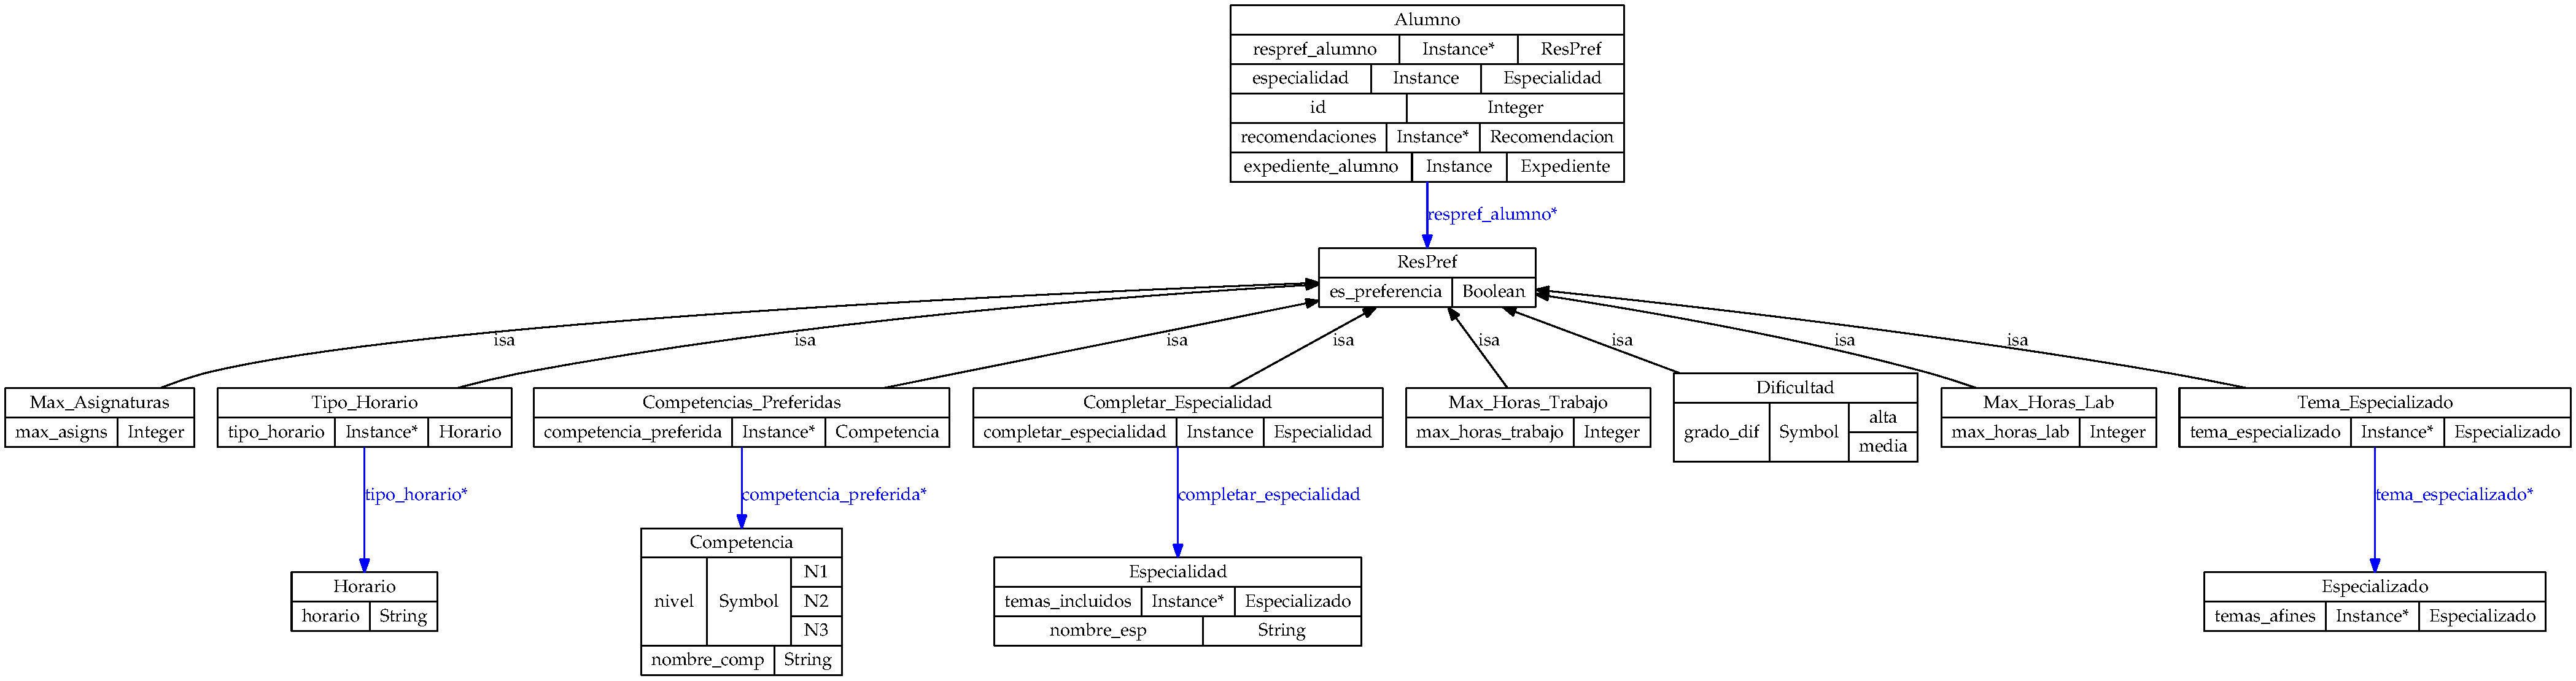
\includegraphics[width=15cm]{ontologia-preferencias}
    \caption{Representación gráfica de la parte de la ontología 
        correspondiente a las preferencias y restricciones.}
    \label{fig:ontologia-preferencias}
\end{figure}

Para poder tener acceso a las preferencias y restricciones, hemos decidido
agruparlos en un solo concepto porque la información que debemos obtener es
la misma para ambas, pero con un matiz distinto en su interpretación. Así, 
pues, creamos una clase \texttt{ResPref} que aglutina restricciones y 
preferencias con un atributo booleano \texttt{es\_preferencia} que nos indica 
si esa determinada condición se ha de cumplir siempre (es decir, se trata de 
una restricción) o si no es algo primordial asegurar su cumplimiento (es 
decir, es simplemente una preferencia). De esta clase se hereda un subconcepto 
para cada tipo de preferencia o restricción que modelamos para que se pueda 
introducir en el sistema. Concretamente, tenemos: \texttt{Max\_Asignaturas}, 
con un atributo \texttt{max\_asigns} que representa un número máximo de 
asignaturas a matricular; \texttt{Max\_Horas\_Trabajo}, con un atributo 
\texttt{max\_horas\_trabajo} que representa el máximo número de horas de 
dedicación semanales a las asignaturas matriculadas; \texttt{Max\_Horas\_Lab}, 
con un atributo \texttt{max\_horas\_lab} que representa el máximo número de 
horas de laboratorio asumibles; \texttt{Dificultad}, con un atributo 
\texttt{grado\_dif} que representa la dificultad de las asignaturas asumible;
\texttt{Tipo\_Horario}, relacionada con \texttt{Horario}, que modela una 
cierta disponibilidad horaria; \texttt{Competencias\_Preferidas}, asociada 
con \texttt{Competencia}, que almacena las competencias transversales 
prioritarias para obtener; \texttt{Completar\_Especialidad}, relacionada con 
\texttt{Especialidad}, que representa la prioridad de completar una cierta 
especialidad con la matrícula; y \texttt{Tema\_Especializado}, relacionada 
con \texttt{Especializado}, que representa los temas de interés del alumno.
De este modo, podremos tener una restricción y una preferencia de cada uno 
de estos subconceptos, y distinguiremos entre ellos gracias a la subclase y 
al booleano \texttt{es\_preferencia}. 
La \autoref{fig:ontologia-preferencias} muestra esta parte de la ontología.

Finalmente, en la \autoref{fig:ontologia-completa} se muestra el esquema 
completo de la jerarquía de la ontología anteriormente descrita.

\afterpage{% Página horizontal (a parte).
\begin{landscape}

    \begin{figure}[ht]
        \centering
        \includegraphics[width=23cm,height=14cm,keepaspectratio]%
            {ontologia-completa}
        \caption{Representación gráfica de la ontología completa.}
        \label{fig:ontologia-completa}
    \end{figure}

\end{landscape}
}

La ontología mostrada es el resultado final de un proceso de diseño iterativo: 
partiendo de un modelo inicial que incluía los elementos más importantes, se 
han ido añadiendo los elementos y características que se han considerado 
necesarias a lo largo del desarrollo de la práctica. 

Antes de empezar con el diseño de la ontología en sí, se hizo un detallado 
análisis del problema (que se puede apreciar en parte de la 
\autoref{sec:conceptualizacion}) para identificar los principales conceptos 
del dominio que resultarían importantes para la resolución del problema. 
Partiendo de estos, empezamos a diseñar las clases de la ontología. En esta 
fase, combinamos una aproximación \textit{de arriba a abajo} (es decir, 
empezamos colocando los conceptos más importantes, representados por clases 
como \texttt{Alumno} o \texttt{Asignatura}, siguiendo con las 
especializaciones de estos) con una aproximación \textit{de abajo a arriba} 
(para las restricciones y preferencias, empezamos con los tipos que queríamos 
representar y decidimos posteriormente aglutinarlas en una clase 
\texttt{ResPref}). Una vez establecidas las clases principales y su jerarquía, 
fuimos añadiendo los atributos que definen las características importantes 
de cada clase y las relaciones entre instancias de las clases, siguiendo el 
análisis de los requerimientos del problema para incluir precisamente aquello 
que consideramos necesario (puesto que, en este caso particular, no se espera 
reaprovechar la ontología para resolver otros problemas en el mismo dominio). 
Finalmente, tras completar el diseño de la ontología propiamente, añadimos las 
instancias de todos aquellos conceptos estrechamente relacionados con el plan 
de estudios del grado (asignaturas, competencias transversales, ...) y, a 
medida que avanzamos en el desarrollo, añadimos instancias con expedientes de 
alumnos ficticios para los juegos de prueba.

La primera versión de la ontología se completó en una fase muy temprana del 
desarrollo de la práctica. A lo largo de este desarrollo, sin embargo, la 
ontología ha sufrido ligeras modificaciones para adaptarse a cambios debidos 
a una mayor comprensión de la especificación del problema. 

La información necesaria para crear las instancias de asignaturas acordes a la 
realidad han sido obtenidos del acta académica publicada por la FIB sobre el 
curso 2013--2014 (la última disponible en el momento de redacción de este 
documento).




